\section{Design}
\label{sec:Design}

\subsection{Overview} 
NeuraViz follows a fairly standard server-client web application architecture. The client is responsible for rendering the user interface and allowing the user to interact with the application. The server handles the actual computationally intensive processes such as parsing the uploaded model and generating the structure of the visual representation. The server also handles the storage of the uploaded models during user sessions. It also handles translation of the visualization into various formats.

\subsection{UML Class Diagram}
The UML class diagram in Figure \ref{fig:uml_class_diagram} shows the classes and their relationships in the NeuraViz application. The diagram is divided into two main sections: the frontend and the backend, which are also commonly referred to as the client and server respectively. 

\begin{figure}[h]
    \centering
    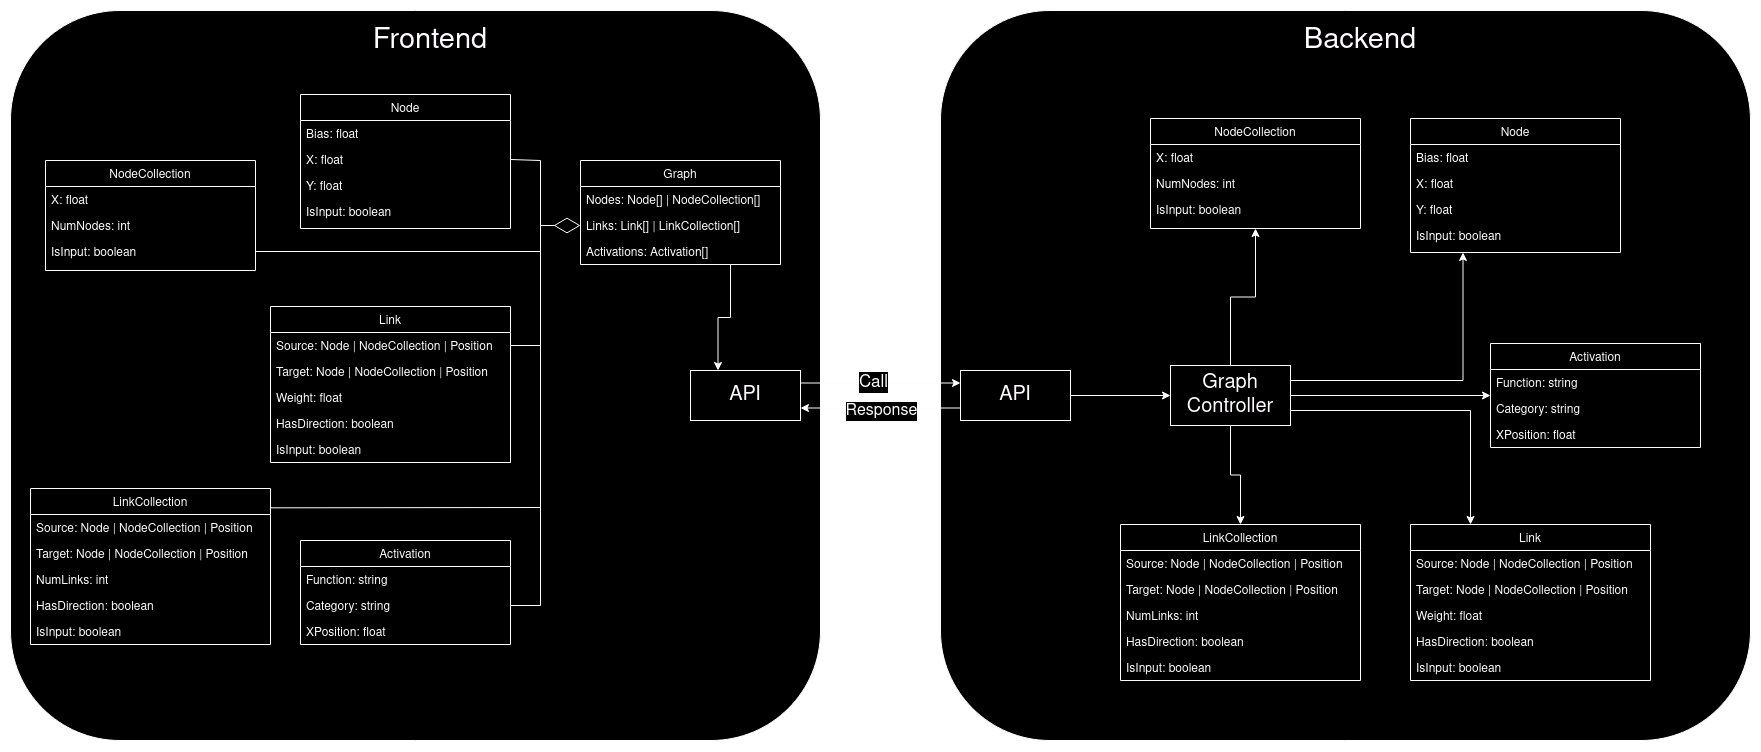
\includegraphics[width=0.8\textwidth]{../docs/diagrams/class_diagram.png}
    \caption{UML Class Diagram}
    \label{fig:uml_class_diagram}
\end{figure}

\subsubsection{Frontend/Client}
The frontend primarily relies on the Graph object, which is comprised of a number of Nodes and/or Node Collections, Links and/or Link Collections, and Activation Functions. Nodes represent individual nodes as represented in the graph, and these are used for nodes in graph layers that are smaller than 10 nodes by default. For layers that are too large, the graph representation instead contains a Node Collection that represents the layer as a whole. Links and Link Collections operate a similar way. Activation Function objects represent the activation functions that can be seen as small icons at the top of each layer in the NeuraViz interface. The graph object houses the representation of the neural network model as ready for rendering. As shown in the UML diagram, the frontend also houses an API component that is responsible for communicating with the backend architecture via standard HTTP requests.

\subsubsection{Backend/Server}
The backend is responsible for handling the computationally intensive processes of parsing the uploaded model and generating the structure of the visual representation. As seen in Figure \ref{fig:uml_class_diagram}, the backend houses objects that almost perfectly mirror the frontend components. However, on the server, these components are all related to the graph controller: the component responsible for the actual graph parsing. In addition to parsing the actual graph, the controller also handles additional requests for retrieving a stored model and converting the representation into various formats. Like with the frontend portion of the application, the backend houses an API component that is responsible for receiving the HTTP requests from the client and routing them to the correct controller endpoint for processing, as well as sending the response back to the client.

\subsection{Database}
% TODO: Add Database

\subsection{User Interface}
% TODO: Add User Interface
